\documentclass[12pt,a4paper]{article}
	%[fleqn]		%% --to make all equation left-algned
\usepackage[top=2in, bottom=1in, left=1in, right=1in]{geometry}
%\usepackage{fullpage}

\usepackage{fancyhdr}\pagestyle{fancy}\rhead{Stephanie Wang}\lhead{Guild to Math151B discussions}

\usepackage{amsmath,amssymb,amsthm,amsfonts,microtype,stmaryrd}
	%{mathtools,wasysym,yhmath}

\usepackage[usenames,dvipsnames]{xcolor}\newcommand{\blue}[1]{\textcolor{blue}{#1}}\newcommand{\red}[1]{\textcolor{red}{#1}}\newcommand{\gray}[1]{\textcolor{gray}{#1}}
\newcommand{\fgreen}[1]{\textcolor{ForestGreen}{#1}}

%\usepackage{mdframed}
	%\newtheorem{mdexample}{Example}
	%\definecolor{warmgreen}{rgb}{0.8,0.9,0.85}
	% --Example:
	% \begin{center}
	% \begin{minipage}{0.7\textwidth}
	% \begin{mdframed}[backgroundcolor=warmgreen, 
	% skipabove=4pt,skipbelow=4pt,hidealllines=true, 
	% topline=false,leftline=false,middlelinewidth=10pt, 
	% roundcorner=10pt] 
	%%%% --CONTENTS-- %%%%
	% \end{mdframed}\end{minipage}\end{center}	

\usepackage{graphicx} \graphicspath{{}}
	% --Example:
	% \includegraphics[scale=0.5]{picture name}

%\usepackage{hyperref}\hypersetup{linktocpage,colorlinks}\hypersetup{citecolor=black,filecolor=black,linkcolor=black,urlcolor=black,breaklinks=true}

%%% --Text Fonts
%\usepackage{times} %%% --Times New Roman for LaTeX
%\usepackage{fontspec}\setmainfont{Times New Roman} %%% --Times New Roman; XeLaTeX only

%%% --Quick Arrows
\newcommand{\ra}[1]{\ifnum #1=1\rightarrow\fi\ifnum #1=2\Rightarrow\fi\ifnum #1=3\Rrightarrow\fi\ifnum #1=4\rightrightarrows\fi\ifnum #1=5\rightleftarrows\fi\ifnum #1=6\mapsto\fi\ifnum #1=7\iffalse\fi\fi\ifnum #1=8\twoheadrightarrow\fi\ifnum #1=9\rightharpoonup\fi\ifnum #1=0\rightharpoondown\fi}
%\newcommand{\la}[1]{\ifnum #1=1\leftarrow\fi\ifnum #1=2\Leftarrow\fi\ifnum #1=3\Lleftarrow\fi\ifnum #1=4\leftleftarrows\fi\ifnum #1=5\rightleftarrows\fi\ifnum #1=6\mapsfrom\ifnum #1=7\iffalse\fi\fi\ifnum #1=8\twoheadleftarrow\fi\ifnum #1=9\leftharpoonup\fi\ifnum #1=0\leftharpoondown\fi}
%\newcommand{\ua}[1]{\ifnum #1=1\uparrow\fi\ifnum #1=2\Uparrow\fi}
%\newcommand{\da}[1]{\ifnum #1=1\downarrow\fi\ifnum #1=2\Downarrow\fi}

%%% --Quick Editor Config
\newcommand{\nid}{\noindent}
\newcommand{\dps}{\displaystyle}

\newcommand{\onum}[1]{\raisebox{.5pt}{\textcircled{\raisebox{-1pt} {#1}}}}
\newcommand{\claim}[1]{\underline{``{#1}":}}
\newcommand{\prob}[1]{{\bf {#1}}}

%%% --Quick Math Mode Config
\renewcommand{\l}{\left}\renewcommand{\r}{\right}
\newcommand{\casebrak}[2]{\left \{ \begin{array}{l} {#1}\\{#2} \end{array} \right.}
\newcommand{\casedef}[4]{\left \{ \begin{array}{ll} {#1} & {#2}\\{#3} & {4} \end{array} \right.}
%\newcommand{\ttm}[4]{\l[\begin{array}{cc}{#1}&{#2}\\{#3}&{#4}\end{array}\r]} %two-by-two-matrix
%\newcommand{\tv}[2]{\l[\begin{array}{c}{#1}\\{#2}\end{array}\r]}
\let\italiccorrection=\/
\def\/{\ifmmode\expandafter\frac\else\italiccorrection\fi}

%%% --Special Math Characters
\def\R{\ifmmode\mathbb R\fi}
\def\N{\ifmmode\mathbb N\fi}
\let\slashedO=\O	% put the value of \O at this line to \slashedO
\def\O{\ifmmode\mathcal O\else\slashedO\fi}	% whenever \O is called it will evaluate the following expression
% although \newcommand does the same thing as \def, it throws error when overwriting existing command; 

%%% --General Math Symbols/Operators
\newcommand{\bc}{\because}
\newcommand{\tf}{\therefore}

\newcommand{\INT}[2]{\int_{#1}^{#2}}
\newcommand{\SUM}[2]{\sum\limits_{#1}^{#2}}
\newcommand{\PROD}[2]{\prod\limits_{#1}^{#2}}
\newcommand{\CUP}[2]{\bigcup\limits_{#1}^{#2}}
\newcommand{\CAP}[2]{\bigcap\limits_{#1}^{#2}}
\newcommand{\SUP}[1]{\sup\limits_{#1}}

%\renewcommand{\o}{\circ}
%\newcommand{\x}{\times}
%\newcommand{\ox}{\otimes}

%%% --Analysis Symbols
\newcommand{\pd}[2]{\frac{\partial{#1}}{\partial{#2}}}
% \newcommand{\UPINT}{\bar\int}
% \newcommand{\UPINTRd}{\overline{\int_{\bb R ^d}}}
% \newcommand{\SUP}[1]{\sup\limits_{#1}}
% \newcommand{\INF}[1]{\inf\limits_{#1}}

%%% --Numericals Symbols
\DeclareMathOperator*{\argmin}{arg\,min}
\DeclareMathOperator*{\argmax}{arg\,max}
\newcommand{\dt}{\Delta t}
%\newcommand{\nxt}{^{n+1}}
%\newcommand{\pvs}{^{n-1}}
%\newcommand{\hfnxt}{^{n+\frac12}}

%%% --Matrix Analysis Symbols
\def\tr{\text{tr}}
\def\vA{\mathbf{A}}
\def\vB{\mathbf{B}}\def\cB{\mathcal{B}}
\def\vC{\mathbf{C}}
\def\vD{\mathbf{D}}
\def\vE{\mathbf{E}}
\def\vF{\mathbf{F}}\def\tvF{\tilde{\mathbf{F}}}
\def\vG{\mathbf{G}}
\def\vH{\mathbf{H}}
\def\vI{\mathbf{I}}\def\cI{\mathcal{I}}
\def\vJ{\mathbf{J}}
\def\vK{\mathbf{K}}
\def\vL{\mathbf{L}}\def\cL{\mathcal{L}}
\def\vM{\mathbf{M}}
\def\vN{\mathbf{N}}\def\cN{\mathcal{N}}
\def\vO{\mathbf{O}}
\def\vP{\mathbf{P}}
\def\vQ{\mathbf{Q}}
\def\vR{\mathbf{R}}
\def\vS{\mathbf{S}}
\def\vT{\mathbf{T}}
\def\vU{\mathbf{U}}
\def\vV{\mathbf{V}}
\def\vW{\mathbf{W}}
\def\vX{\mathbf{X}}
\def\vY{\mathbf{Y}}
\def\vZ{\mathbf{Z}}

\def\va{\mathbf{a}}
\def\vb{\mathbf{b}}
\def\vc{\mathbf{c}}
\def\vd{\mathbf{d}}
\def\ve{\mathbf{e}}
\def\vf{\mathbf{f}}
\def\vg{\mathbf{g}}
\def\vh{\mathbf{h}}
\def\vi{\mathbf{i}}
\def\vj{\mathbf{j}}
\def\vk{\mathbf{k}}
\def\vl{\mathbf{l}}
\def\vm{\mathbf{m}}
\def\vn{\mathbf{n}}
\def\vo{\mathbf{o}}
\def\vp{\mathbf{p}}
\def\vq{\mathbf{q}}
\def\vr{\mathbf{r}}
\def\vs{\mathbf{s}}
\def\vt{\mathbf{t}}
\def\vu{\mathbf{u}}
\def\vv{\mathbf{v}}\def\tvv{\tilde{\mathbf{v}}}
\def\vw{\mathbf{w}}
\def\vx{\mathbf{x}}\def\tvx{\tilde{\mathbf{x}}}
\def\vy{\mathbf{y}}
\def\vz{\mathbf{z}}


%%%%%%%%%%%%%%%%%%%%%%%%%%%%%%%%%%%%%%%%%%%%%%%%%%%%%%%%%%%%%%%%%%%%%%%%%%%%%%%%%%%%%%%%%%%%%%%%%%%%%%%%%%%%%%%%%%%%%%%%%%%%%%%%%%%%%%%%%%%%%%%%%%%%%%%%%%%%%%%%%%%%%%%%%%%%%%%%%%%%%%%%%%%%%%%%%%%%%%
\begin{document}
\begin{enumerate}
\item IVP (theoreticals)
	\begin{enumerate}
	\item Some sample IVPs, e.g. $y' = \lambda y$, Hamiltonian systems, $y' = \/y{1-y^2}, y(0) = 0$
	\item Lipschitz Condition (analyze some examples)
	\item Well-posedness and its importance
	\item Theorem: Continuity + Lipschitz condition $\ra2$ well-posedness
	\end{enumerate}
\item Euler's Method
	\begin{enumerate}
	\item Sample problem $y' = \lambda y$
	\item Graphical interpretations
	\item Local truncation error
	\item $y(t_{n+1}) = y(t_n) + \INT{t_n}{t_{n+1}} f(s, y(s))ds$. General methods can be derived by approximating the integral
	\end{enumerate}
\item Taylor's Method
	\begin{enumerate}
	\item Sample problem $y' = ye^t, y(0) = 1$
	\item Taylor expansion with 2 variables
	\item Big O notations
	\end{enumerate}
\item RK
	\begin{enumerate}
	\item Midpoint Method (\& it's local truncation error)
	\item Consistency formula (\& higher order formula)
	\item Butcher tableau
	\item Stability = continuity + Lipschitz condition
	\end{enumerate}
\item Multistep Methods
	\begin{enumerate}
	\item Proper formulation of multiple Taylor expansions
	\item Consistency formula (\& higher order formula)
	\item $y(t_{n+1}) = y(t_n) + \INT{t_n}{t_{n+1}} f(s, y(s))ds$; quadrature rules help approximate the integral
	\item Newton backward-difference formula 
	\begin{center}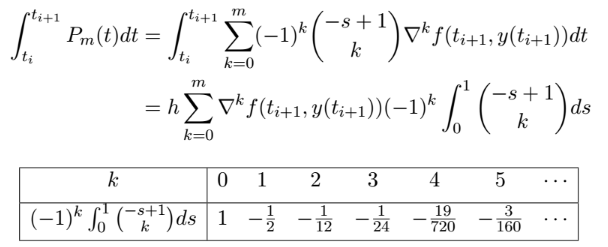
\includegraphics[scale=0.5]{NewtonBackwardDiffFormula.png}\end{center}
	\item Stability = root condition (+ continuity + Lipschitz condition)
	\item Lax equivalence
	\end{enumerate}
\item Stiff Equations, BVPs
	\begin{enumerate}
	\item Region of absolute stability
	\item A-stability
	\item E \& U for solutions to BVPs
	\item Shooting method (linear \& nonlinear)
	\item Finite difference method
	\end{enumerate}
\item Nonlinear System Solvers
	\begin{enumerate}
	\item Fix-point method
	\item Newton's method
	\item (Broydent's method)
	\item Steepest descent method
	\item Homotopy method
	\item (find textbook problems, derive derivatives, and explain the concepts)
	\end{enumerate}
\item Eigen Problems (Power Method, QR-Algorithm)
	\begin{enumerate}
	\item Diagonalizablility conditions
	\item Norms are all equivalent
	\item Shifted inverse power method
	\item Householder transformation and its graphical interpretations and examples
	\item Why does Gram-Schmidt suck? $v_1 = (1,\epsilon,0,0), v_2 = (1,0,\epsilon,0), v_3 = (1,0,0,\epsilon)$
	\end{enumerate}
\item Fast Fourier Transform
	\begin{enumerate}
	\item ???
	\end{enumerate}
\end{enumerate}

\end{document}
